\documentclass[runningheads,a4paper]{llncs}
\usepackage{amssymb}
\setcounter{tocdepth}{3}
\usepackage{listings}
\usepackage{booktabs}
\usepackage{mathtools}
\usepackage{tabularx}
\usepackage{fixltx2e}
\PassOptionsToPackage{hyphens}{url}\usepackage{hyperref}
\usepackage[hyphens]{url}
\usepackage{upquote,textcomp}
\lstset{breaklines=true, basicstyle=\scriptsize\ttfamily, upquote=true}

\usepackage{fancyvrb}
\VerbatimFootnotes
\usepackage{cprotect}

\usepackage{graphicx}
\makeatletter
\def\maxwidth#1{\ifdim\Gin@nat@width>#1 #1\else\Gin@nat@width\fi}
\makeatother

\usepackage{amsmath}
\usepackage{pmml-new}

\usepackage{color,graphics,array,csscolor}

\usepackage{fontspec,unicode-math}
\usepackage[Latin,Greek]{ucharclasses}
\setTransitionsForGreek{\fontspec{Times New Roman}}{}

\usepackage{subscript}
\lstset{breaklines=true, basicstyle=\scriptsize\ttfamily}

\begin{document}
\mainmatter

\title{A semantic approach to recognize behaviours in teenagers}
\titlerunning{A semantic approach to recognize behavi}
\author{Gianfranco E. Modoni\inst{1} \and
Marco Sacco\inst{2} \and
Gabriela Candea\inst{3} \and
Silvia Orte\inst{4} \and
Filip Velickovski\inst{4}}
\authorrunning{Gianfranco E. Modoni et al.}
\institute{Institute of Industrial Technologies and Automation - National Research Council, Bari, Italy\and
Institute of Industrial Technologies and Automation - National Research Council, Milano, Italy\and
Ropardo S.R.L., Sibiu, Romania\and
Eurecat, Barcelona, Spain\\
\email{gianfranco.modoni@itia.cnr.it, 
marco.sacco@itia.cnr.it, 
gabriela.candea@ropardo.ro, 
silvia.orte@eurecat.org, 
filip.velickovski@eurecat.org}}
\maketitle

\begin{abstract}
This research aims to realize a knowledge-based system recognizing teenagers' behaviours in the lifestyle domain. Since various heterogeneous data sources are involved in this recognition process (e.g. wearable sensors, etc.), it is essential to face the harmonization of the data produced from these disparate sources and expressed under the form of both structured and unstructured content. The herein proposed approach leverages a common semantic reference model which represents the individual as a whole, permitting classification and integration of behavioural and contextual information. In this regard, an automatic semantic enrichment of the data produced by the involved sources is carried out, thus allowing to support a behaviour recognition process handled in a two-phase process (real-time and long-term detection and analysis of behaviours and trends).

\keywords{Behaviour recognition, Context awareness, Semantic Repository, Semantic Web}
\end{abstract}


\section{Introduction}

Presently we are witnessing a growing demand of customized services which are tailored to the specific needs and characteristics of users. A key success factor for the implementation of these services is the user profiling, which consists of creating an explicit representation of a person's identity, i.e., a conceptual understanding of the user  \cite{_Ref490677013} \cite{_Ref490677039} that is commonly employed to enhance usability as well as to support personalization, adaptivity and other user-centric features  \cite{_Ref490677081}. In addition, as a user might be found in various contexts, it is essential to construct a conceptual representation of a user model which is context-aware, thus able to infer which context the user is in a given moment in time, and consequently adapts the intervention to the selected context.  

This paper reports major features of an approach to support the process of user profiling which leverages the combination of Semantic Web technologies (SWT)  \cite{_Ref490677097} with the mobile and wearable technologies. The potential of this approach has been verified in the context of the European research project PEGASO\footnote{\url{http://pegasof4f.eu/home}} \cite{_Ref490677114} which aimed at promoting healthy lifestyle among teenagers. In particular, it provides personalized interventions based on the recognition of users' behaviours with the objective of triggering an adjustable behaviour change process. In this regard, an ontology-based approach (Fig. 1)  \cite{_Ref490677130} is adopted to capture and cover the knowledge related with the so called Virtual Individual Model (VIM)  \cite{_Ref490677147}, characterizing the user on different aspects (i.e. physical, functional and behavioural parameters)  \cite{_Ref490677160}. Such a common reference model, which represents the individual as a whole, can contribute to harmonize data from different sources, providing in this way a systematic manner to classify and integrate the valuable knowledge. In fact, the common data model collects all the information and defines the reciprocal relationships between individual's different aspects, aggregating and unifying all the information. The definition of VIM stems from a conceptual framework of relations linking status, behaviours of the individual in different domains as well the context and the relation  \cite{_Ref490677173}.  

This paper is structured as follows. Section 2 introduces the behaviour recognition in PEGASO project, while Section 3 illustrates the semantic approach followed in this project to support behaviour recognition. Finally, Section 4 draws the conclusions, summarizing the main outcomes.
\begin{figure}[h!]
\centering
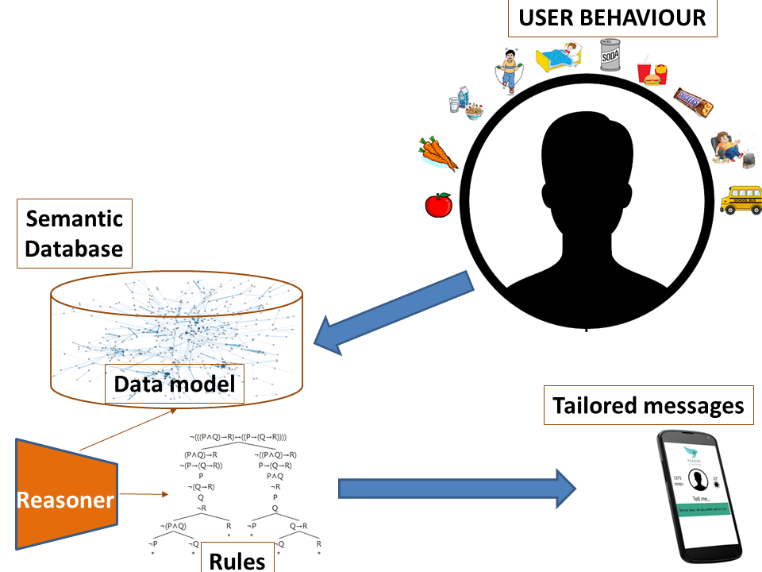
\includegraphics[width=\maxwidth{\textwidth}]{./img/image1.png}
\cprotect\caption{PEGASO approach based on Semantic Web Technologies}
\label{}
\end{figure}


\section{The behaviour recognition in PEGASO}

\subsection{The data sources }

Leveraging the VIM, a Behaviour Recognition System (BRS) has been implemented to conduct an individualized behaviour detection. The BRS is implemented as a two-dimensional system (short and long term) to be able to measure the two timescales considered in the project. In particular, the BRS is based on a mobile platform, where the smartphone is a key element that acts as the main contact point with the user. The mobile device also acts as communication gateway towards the sensors, running reasoning processes that allows inferring in real-time the necessary information to personalize the interventions delivered through the apps. This analysis is performed upon the available data extracted from various sources. Specifically:
\begin{itemize}
\item Physical activity and sleep data is retrieved from available wearables (e.g. bracelet, etc.) and smartphone accelerometer.  
\item Nutritional information is gathered through a mobile food app. 
\item Context data includes different kind of information that involves users' situation in a certain moment (e.g. day and weather information, user location).
\end{itemize}

\section{Overview of the Knowledge Based System}

\subsection{The VIM ontology}

The definition of a common reference model, which represents the individual as a whole, is proposed as a solution to harmonize data from the different heterogeneous sources, providing in this way a systematic manner to classify and integrate the valuable knowledge. The common data model defines the reciprocal relationship between the individual's different aspects, aggregating and unifying all this information. In particular, the definition of such virtual individual model stems from a conceptual model of relations linking status, behaviours of the individual in different domains as well the context surrounding the individual. This reference model is represented through a set of ontologies by adopting the SWT. An ontology based approach offers the significant key advantages of allowing to represent a formal semantics which contributes to enhance the interoperability of different software applications. In addition, it allows to entail and infer new knowledge about the concepts and their linking relationships, in addition to those initially already asserted. Finally, it allows to efficiently model and manage data to be distributed over the network, under the form of Linked Open Data (LOD)  \cite{_Ref490677234}. The latter is a proven way to publish and interlink public set of data in the scientific community (and also other fields).  Considering the relevance of the open model, we could imagine another connection to the LOD diagram through a circle containing the VIM meta model which is paired with a data set of example.

\subsection{The architecture}

The proposed technological architecture is capable to handle and expose the VIM ontology (expressed in OWL DL\footnote{ http://www.w3.org/TR/owl-features/}). It consists of two main pillars hosted on AWS cloud: the Semantic Repository (SR) and the Connector (Fig. 2). This latter represents the one single gateway, which play the role of Integration Service  \cite{_Ref490677244}, by transforming and combining structured and unstructured legacy data into valuable information according to the common data model behind VIM ontology. After this conversion process, the extracted information are also persisted and stored in a specific database (Semantic Repository). Specifically, the managed data comprise (Figure 3): 
\begin{itemize}
\item the domain ontology (TBOX), as representation of the knowledge about VIM; 
\item the ontological population (ABOX), compliant to the domain ontology; 
\item the derivation rules (RBOX) needed to properly entail the implicit knowledge and specified through the syntax of SWRL\footnote{\url{https://www.w3.org/Submission/SWRL/}}.
\end{itemize}

The Connector, exposed as a RESTFUL web-service, is in charge of translating received HTTP requests into corresponding queries, formulated in SPARQL\footnote{\url{https://www.w3.org/TR/sparql11-query/}} which is the standard language to compose the semantic query. Thus, SPARQL queries play the role of mediator between the application-driven models and the ABOX, TBOX and RBOX of the VIM model (Fig. 3).  

\subsection{The Semantic Repository}

One of the strengths of the SWT is that they allow to virtually express any type of information. The flip side is that this expressivity and flexibility imply the need to revise for SWT most part of the classical data management problems, including efficient storage and query optimization. Thus, as the request of semantic applications in real scenarios is continuously growing, the issue of efficiently storing and retrieving RDF data is getting more and more relevant. This need is posing significant challenges for researchers and technologists in terms of scalable and efficient stores. Under these conditions, a significant study of the PEGASO project has regarded the identification of a valid RDF store  \cite{_Ref490721446}, which finally brought to exploit an instance of the Stardog database\footnote{\url{http://stardog.com/}}.

\subsection{Interaction of the data sources with the Semantic Repository}

BRS takes advantage of both mHealth (smartphone apps and wearables) and cloud solutions to perform a two-stage processing of the user-generated data at different timespans to provide different levels of feedback and user interaction. Collected data, which encompasses indicators of detectable target behaviours, is cleaned and then fused into daily aggregated summaries (24h timespan) that are finally stored in the SR deployed in the cloud for further knowledge management. Additionally, collected and inferred data in those 24h timespan is continuously analyzed to provide real-time response to detected events such as behaviour abnormalities.

On the other side, the PEGASO cloud consumes the inferred information from the semantic repository to build a longer timespan summary (1 month) to be further analyzed. This long-term analysis is in charge of identifying user behaviour trends and evaluate the user progression on the goals set in the platform. As a result, it provides behavioural feedback and recommendations on personalized behaviour change interventions.


\begin{figure}[h!]
\centering

\includegraphics[width=\maxwidth{\textwidth}]{./img/image2.png}
\cprotect\caption{Technological platform hosting VIM ontology}
\label{}
\end{figure}

\begin{figure}[h!]
\centering
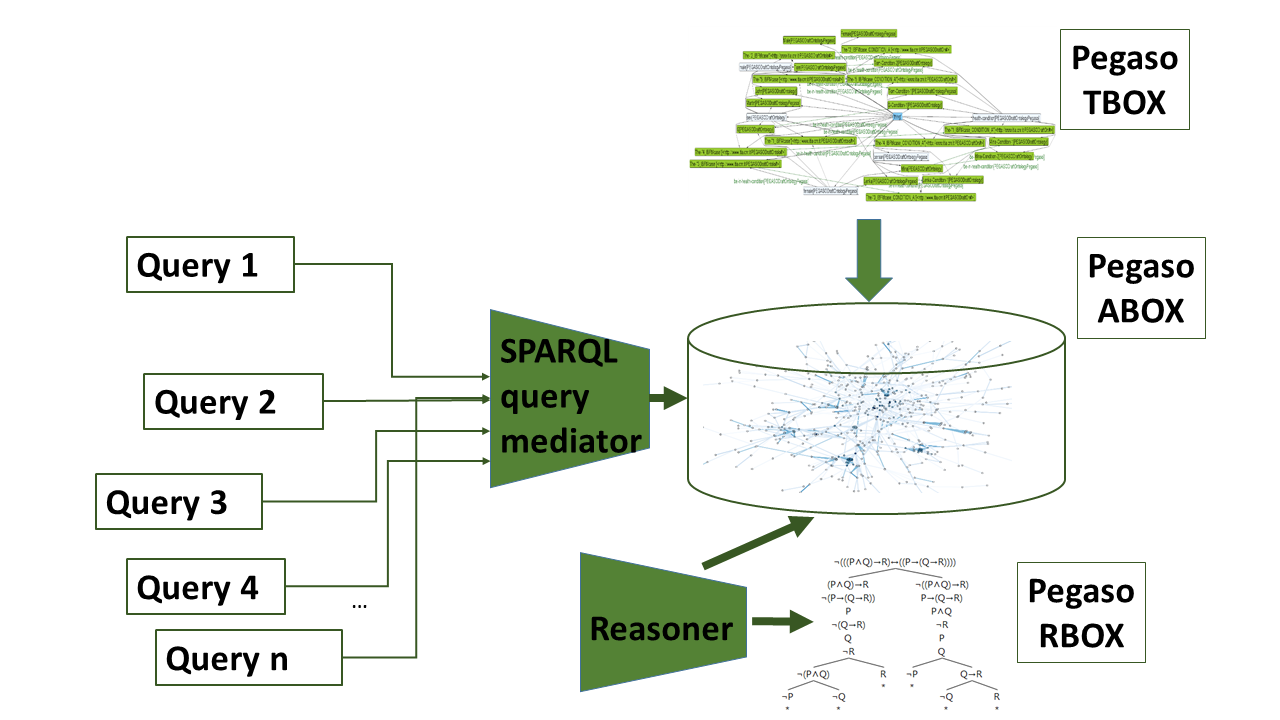
\includegraphics[width=\maxwidth{\textwidth}]{./img/image3.png}
\cprotect\caption{  Ontology querying mechanism}
\label{}
\end{figure}


\section{Experimental Settings}

The services exposed by the architecture had been evaluated in terms of performance under  heavy load (e.g high number of client connections), through a session of  stress tests, using the Chrome plugin RESTful Stress\footnote{\url{https://chrome.google.com/webstore/detail/restful-stress/}}. The stress test demonstrated that the overall architecture satisfies the requirement in terms of horizontal scalability. Moreover, a six-month pilot study to assess the feasibility of the system in real life conditions was carried out in four different countries. Approximately 350 participants of the four pilot sites have been involved during the study. The feedback concerning the use of the semantic architecture is positive. In particular, the architecture confirmed its capability to support the concurrent access of different users (up to 100) with an acceptable average duration of a request (under the threshold of 100 milliseconds). 

\section{Conclusions}

This paper has introduced an approach to support teenager behaviour recognition which is based on a semantic architecture. The latter offers interesting advantage, in particular allowing to enhance the semantic interoperability of the data sources monitoring and collecting teenager data. In addition, the architecture provides a SPARQL endpoint, which is the preliminary step to expose the meta-model of the VIM as Linked Open Data.  

Future developments will address three main goals. First of all, the VIM-based approach will be validated also with other categories of users, different from teenagers (e.g. elderly people or people with impairment). In fact, even the PEGASO approach has been conceived for teenager, VIM ontology can be tailored for other categories of users, while the semantic architecture is agnostic to the meta-model  of the used semantic data. The second goal will concern the integration of other sensors to extend the functionalities of the already implemented knowledge based system. Finally, the proposed architecture will be extended to enable a new model of collaboration among the involved sensors and apps, which can support their synergistic and smarter interaction and cooperation  \cite{_Ref490756416}. 

\subsubsection*{Acknowledgements.}This work has been partially funded by the EU 7th Framework Programme under the grant agreement No: 610727, ``Personalised Guidance Services for Optimising lifestyle in teenagers through awareness, motivation and engagement'' (PEGASO).


\begin{thebibliography}{4}

\bibitem{_Ref490677173} A. Sojic, W. Terkaj, et al.. Modularising ontology and designing inference patterns to personalise health condition assessment: the case of obesity. Journal of Biomedical Semantics, 7(1), 12, 2016.
\bibitem{_Ref490677234} C. Bizer, T. Heath, and T. Berners-Lee. Linked data-the story so far. Semantic Services, Interoperability and Web Applications: Emerging Concepts, 2009.
\bibitem{_Ref490677147} C. Lafortuna, J. C. Serrano, et al.. The building of a virtual individual model (VIM): multi domain characterisation of health status in the PEGASO project. Advances in Human Aspects of Healthcare, 2014.
\bibitem{_Ref490677160} F. Velickovski, S. Orte, et al.. Detection and Assessment of Behaviours Associated with the Risk of Obesity in Adolescents. In eHealth 360°. Springer International Publishing, 2017.
\bibitem{_Ref490721446} G. E. Modoni, M. Sacco, and W. Terkaj. A survey of RDF store solutions. Proceedings of the 20th International Conference on Engineering, Technology and Innovation, 2014.
\bibitem{_Ref490677244} G. E. Modoni, M. Veniero, and M. Sacco. Semantic Knowledge Management and Integration Services for AAL Applications. Proceedings ForItAAL2016, Lecture Notes in Electrical Engineering, 2016.
\bibitem{_Ref490677039} G. Fischer. User Modeling in Human-Computer Interaction. User Modeling and User-Adapted Interaction. 11: 65-68, 2001.
\bibitem{_Ref490756416} G.E. Modoni, M. Veniero, A. Trombetta, et al.. Semantic based events signaling for AAL systems. Journal of Ambient Intelligence and Humanized Computing, 2017.
\bibitem{_Ref490677081} M. Golemati et al.. Creating an ontology for the user profile: Method and applications. Proceedings of the first RCIS conference, 2007.
\bibitem{_Ref490677013} M. Sacco, E. G. Caldarola, G. Modoni, and W. Terkaj. Supporting the design of AAL through a SW integration framework: the D4All project. International Conference on Universal Access in Human-Computer Interaction. Springer International Publishing, 2014.
\bibitem{_Ref490677114} R. Guarneri, and G. Andreoni. PEGASO Fit for Future. European Project Space on Computational Intelligence. Knowledge Discovery and Systems Engineering for Health and Sports.
\bibitem{_Ref490677097} T. Berners-Lee, J. Hendler and O. Lassila, "The Semantic Web", Scientific American, vol. 284, n. 5, 2001.
\bibitem{_Ref490677130} T. R. Gruber. A translation approach to portable ontology specifications. Knowledge acquisition, 5(2), 1993.

\end{thebibliography}

\end{document}